In conclusion, the higher the fretting position, the more intonation error there is. The relationship is not a linear one but quite complicated and can be modelled with the equation (\ref{eqn33}). By plotting the collected data and performing the goodness-of-fit test, it confirms the validity of the equation. \par
By choosing a simplified model of the guitar, it makes the calculations easier and creates a useful approximation model. However, the model doesn't take into account several factors in reality that can affect the intonation. For example, the use of a capo to simulate the fretting action of a human finger. The contact surface of a human finger on the string is very small, but that of a capo is much bigger. This can lead to more deformation of the string when using the capo and consequently an increase in tension \& frequency. Also, when fretting down on the string we don't normally press down directly on the fret like the capo, but a bit behind. This can depress the string more and lead to a higher intonation error. Another factor is the guitar neck isn't always rigid and straight like in the model but sometimes slightly bowed, either from the tension of the strings or set up by the player, which can also affect the intonation. An assumption I made in the experiment is the point of pressing down on the string would have no friction, therefore the tension increase would be distributed evenly throughout the string, but in reality the finger or the capo would have a small amount of friction that can affect the result. Another limitation of the model is it only applies to plain unwound steel strings, so it can only be used for the highest 3 strings on a guitar, but for the other 3 wound strings we would need a different model.\par

An observation I can make from equation (\ref{eqn33}) is that it is not dependent on the gauge (thickness) of the string I use. However this conflicts with my experience, because when playing I would notice the thicker G string would exhibit more intonation shift than the thinner high E string. The explanation I have for this is due to the different $f_0$ of both strings. For E string tuned to E4, $f_0 = \SI{329.63}{Hz}$. Plotting the graph for this (Figure \ref{fig11}), we see the intonation deviation is much lower than for the G string, as expected.\par
\FloatBarrier
\begin{figure} [!htb]
    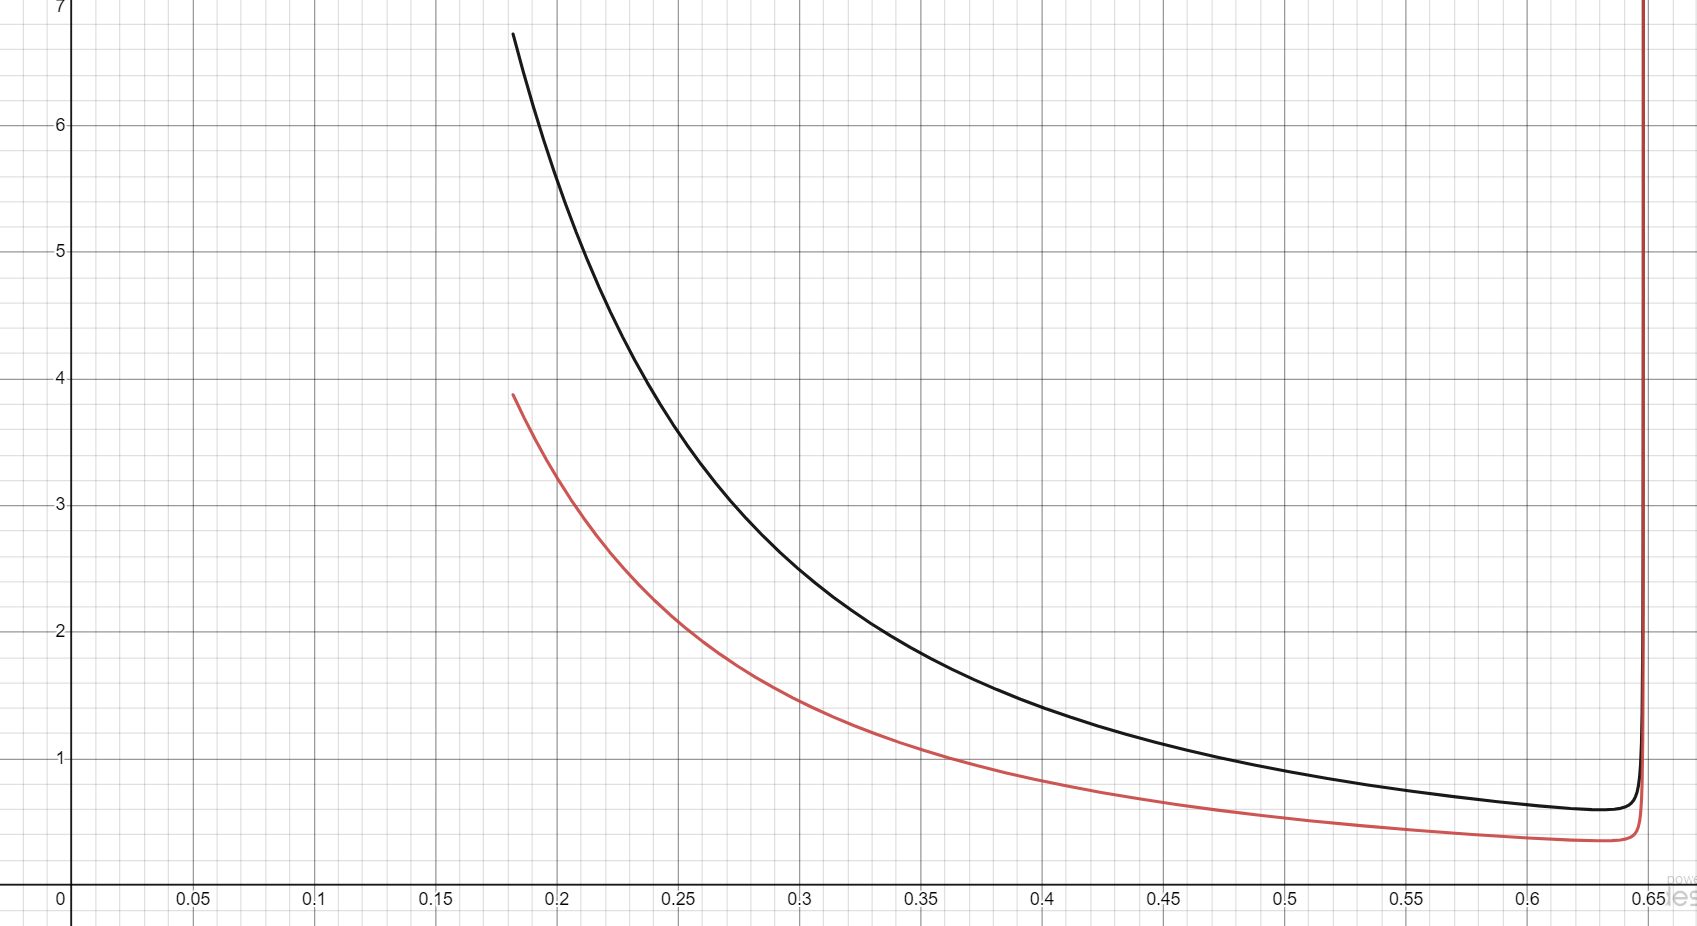
\includegraphics[width = \textwidth]{./ee/compare_graph_f.png} 
    \caption{Comparison of curve for G string (black) and high E string (red)}\label{fig11}
\end{figure}
Another very similar phenomenon often reported among guitar players is that, for the same string, using thicker string gauge would make the intonation a little flat overall. This means $f_0$ and every other variables are the same, but now we have negative values of $\Delta f$. This cannot be explained by the equation or shown in the graph, but I think this is caused by a different factor. For a thicker string, from equation (\ref{eqn4}), in order to tune to the same frequency $f_0$ we would need a higher tension $T$, because the linear density $\mu$ of a thicker string is larger. This higher tension would make it harder to fret down on the string (more "string resistance"), requiring more force, increasing the string tension and bending the neck slightly more. This means the string will get a little slacker and the frequency will go down. Therefore in order to minimize intonation error, it is recommended to use thinner gauge strings. However players need to take into account other factors as well when changing strings. For example it's not recommended for players with a slightly heavier playing style, because the lower resistance of thinner strings will make it more likely to be pushed sideways when fretted rather than directly down on the fret, which will also cause intonation shifts.\par

From the graph of the equation relating $\Delta f$ and $l_n$ we can also evaluate the effects of changing other variables on the shape of the curve. It is impossible to have zero intonation deviation through the whole graph, but I can try ways to minimize this error. I notice the variable that has the most effect on the graph is $a$, the vertical distance between top of the bridge saddle and the frets. Simply reducing the value of $a$ by around 1 mm, bringing it from 3.3 mm down to 2 mm (\SI{2e-3}{m}) is enough to reduce the intonation shift at fret 16 down to around 1.2 Hz (Figure \ref{fig12}), which would be almost unnoticeable to the human ear. \par
\begin{figure}[!h]
    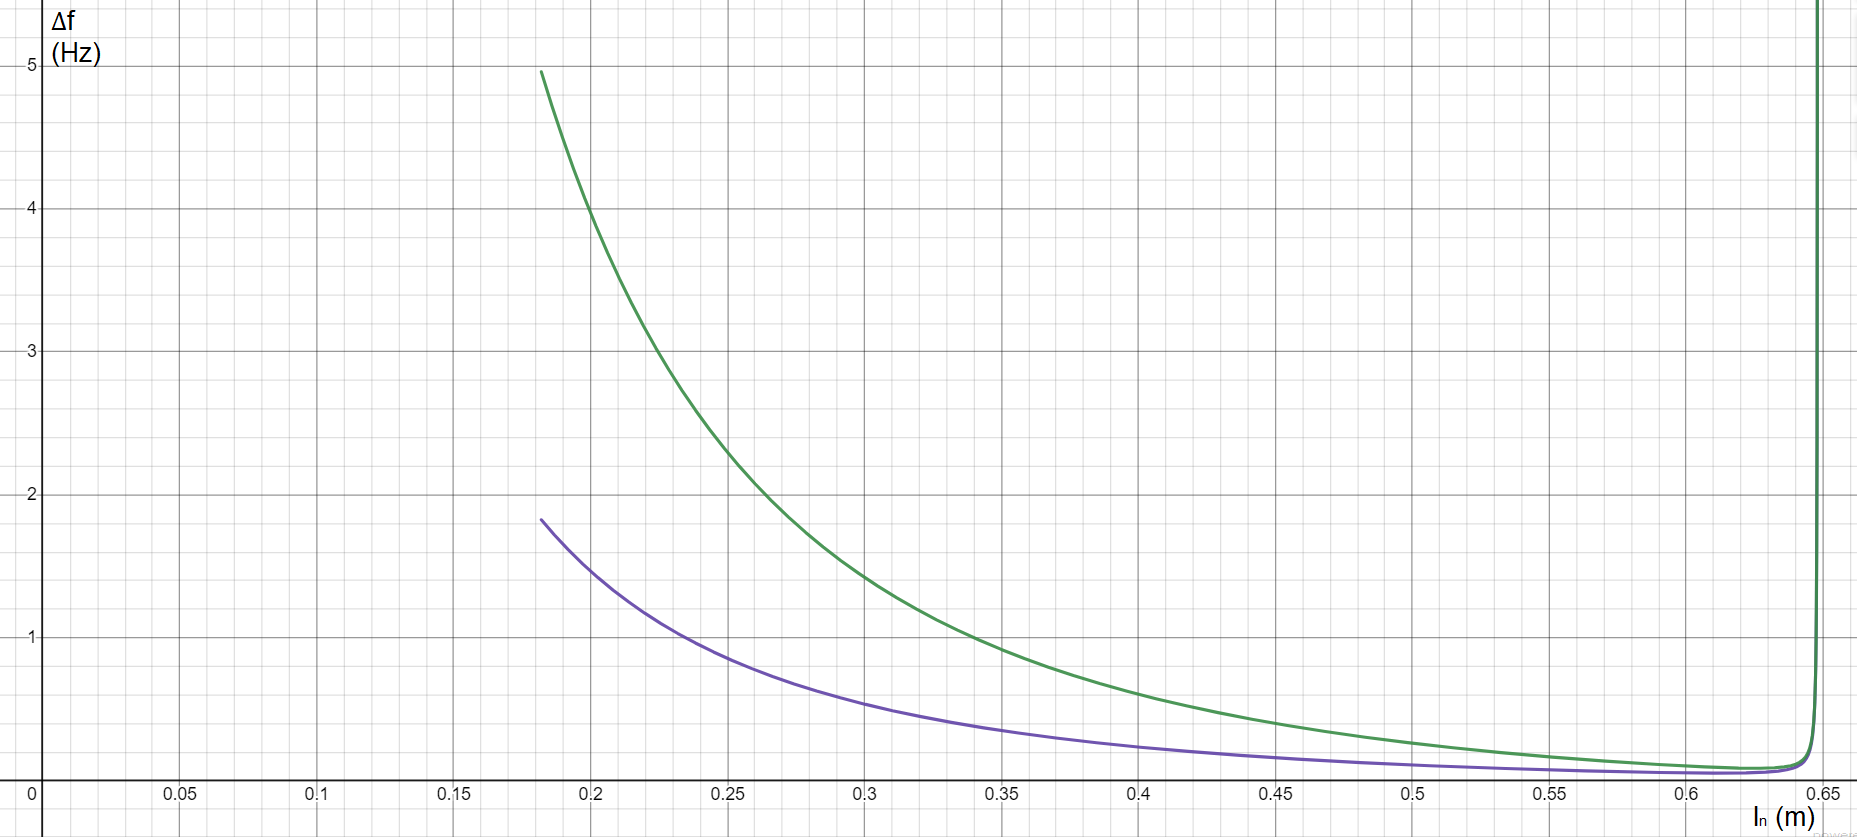
\includegraphics[width = \textwidth]{./ee/compare_graph_a.png}
    \caption{Comparison of before (black) and after changing value of $a$ (red)} \label{fig12}
\end{figure}
\FloatBarrier
So a lower string action would be better for intonation. Guitar manufacturers as well as guitarists can take this into account when setting up their guitars to reduce the intonation error. However, reducing the saddle height too much will cause buzzing of the string, where the string hit against other frets when it is plucked and vibrating. This will reduce the quality of the tone and might even lead to more intonation error. Therefore a careful trial and error approach is needed when adjusting for a good intonation. \par
Overall from the investigation we see that the intonation of a guitar string is a complicated variable and is affected by a lot of different factors. We cannot eliminate it completely, but there are some things we can do to control it to try and minimize the intonation shifts, such as using low gauge strings and having a low action. However I believe guitar players shouldn't worry too much about it, as I think intonation errors generally exhibit "self-correcting" behavior. This is because when a player can hear slight deviations in pitch, their fretting fingers will make micro-movements to try to compensate for this.